\item Consider the marks obtained by 10 students in a mathematics test as given below:\\
42 25 78 75 62 55 36 95 73 60\\
Find the highest and the lowest marks.
\item Consider the marks obtained (out of 100 marks) by 30 students of Class IX of a school.  Draw the freqeuncy distribution table.

%\begin{table}[!ht]
%\centering
%\resizebox{\columnwidth}{!}{
\begin{tabular}{cccccccccc}
10 &20 &36 &92 &95 &40 &50 &56 &60 &70\\
92 &88 &80 &70 &72 &70 &36 &40 &36 &40\\
92 &40 &50 &50 &56 &60 &70 &60 &60 &80\\
\end{tabular}
%}
%\caption{}
%\label{table:2.1.11}
%\end{table}

\item 100 plants each were planted in 100 schools during Van Mahotsava. After one month, the number of plants that survived were recorded as follows.  Draw the grouped distribution table in intervals 20-29, 30-39 etc...

\begin{tabular}{cccccccccc}
95 &67 &28 &32 &65 &65 &69 &33 &98 &96\\
76 &42 &32 &38 &42 &40 &40 &69 &95 &92\\
75 &83 &76 &83 &85 &62 &37 &65 &63 &42\\
89 &65 &73 &81 &49 &52 &64 &76 &83 &92\\
93 &68 &52 &79 &81 &83 &59 &82 &75 &82\\
86 &90 &44 &62 &31 &36 &38 &42 &39 &83\\
87 &56 &58 &23 &35 &76 &83 &85 &30 &68\\
69 &83 &86 &43 &45 &39 &83 &75 &66 &83\\
92 &75 &89 &66 &91 &27 &88 &89 &93 &42\\
53 &69 &90 &55 &66 &49 &52 &83 &34 &36\\
\end{tabular}\\
\item Let us now consider the following frequency distribution in Table \ref{table:2.1.13}
which gives the weights of 38 students of a class.  If two new students of weights 35.5 kg and 40.5 kg are admitted in the class, revise the distribution table accordingly.
\begin{table}[!ht]
\centering
\resizebox{\columnwidth}{!}{
\begin{tabular}{|c|c|}
\hline
\textbf{Weights(in kg)} &\textbf{Number of students}\\
\hline
31-35 &9\\
36-40 &5\\
41-45 &14\\
46-50 &3\\
51-55 &1\\
56-60 &2\\
61-65 &2\\
66-70 &1\\
71-75 &1\\
\hline
\textbf{Total} &38\\
\hline
\end{tabular}
}
\caption{}
\label{table:2.1.13}
\end{table}
\item In a particular section of Class IX, 40 students were asked about the months of their birth and the following graph was prepared for the data so obtained:\\

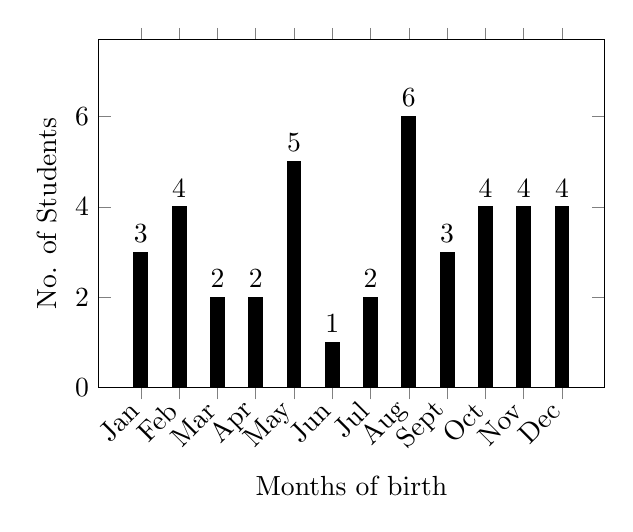
\begin{tikzpicture}
\begin{axis}[
ybar,
ymin=0,
width=8cm,
height=6cm,
ymax=7,
bar width=5pt,
ylabel={No. of Students},
xlabel={Months of birth},
nodes near coords,
symbolic x coords={Jan,Feb,Mar,Apr,May,Jun,Jul,Aug,Sept,Oct,Nov,Dec},
xtick = data,
x tick label style={rotate=45,anchor=east},
enlarge y limits={value=0.1,upper},
legend pos=north east,
],
\addplot[fill=black] coordinates {(Jan,3) (Feb,4)(Mar,2) (Apr,2)(May,5)(Jun,1)(Jul,2)(Aug,6)(Sept,3)(Oct,4)(Nov,4)(Dec,4)};
\end{axis}
\end{tikzpicture}\\

Observe the bar graph given above and answer the following questions:\\

(i) Many students were born in the month of November?\\
(ii)In which month were the maximum number of students born?\\

\item A family with a monthly income of \rupee 20,000 had planned the following
expenditures per month under various heads:\\
\begin{tabular}{|c|c|}
\hline
\textbf{Heads} &\textbf{Expenditure(in 1000\rupee)}\\
\hline
Grocery &4\\
Rent &5\\
Education of children &5\\
Medicine &2\\
Fuel &2\\
Entertainment &1\\
Miscellaneous &1\\
\hline
\end{tabular}\\

Draw a bar graph for the data above.\\

\item A teacher wanted to analyse the performance of two sections of students in a mathematics test of 100 marks. Looking at their performances, she found that a few students got under 20 marks and a few got 70 marks or above. So she decided to
group them into intervals of varying sizes as follows: 0 - 20, 20 - 30, . . ., 60 - 70, 70 - 100. Then she formed the following table:\\
\begin{tabular}{|c|c|}
\hline
\textbf{Marks} &\textbf{Number of students}\\
\hline
0-20 &7\\
20-30 &10\\
30-40 &10\\
40-50 &20\\
50-60 &20\\
60-70 &15\\
70-above &8\\
\hline
\textbf{Total} &90\\
\hline
\end{tabular}\\
\item Consider the marks, out of 100, obtained by 51 students of a class in a test, given in Table.\\
\begin{tabular}{|c|c|}
\hline
\textbf{Marks} &\textbf{No.of Students}\\
\hline

0-10 &5\\
10-20 &10\\
20-30 &4\\
30-40 &6\\
40-50 &7\\
50-60 &3\\
60-70 &2\\
70-80 &2\\
80-90 &3\\
90-100 &9\\
\hline
\textbf{Total} &51\\
\hline
\end{tabular}\\

Draw a frequency polygon corresponding to this frequency distribution table.\\

\item n a city, the weekly observations made in a study on the cost of living index are given in the following table:\\
\begin{tabular}{|c|c|}
\hline
\textbf{Cost of living index} &\textbf{No. of weeks}\\
\hline
140-150 &5\\
150-160 &10\\
160-170 &20\\
170-180 &9\\
180-190 &6\\
190-200 &2\\
\hline
\textbf{Total} &52\\
\hline
\end{tabular}\\

Draw a frequency polygon for the data above (without constructing a histogram).\\
\item 5 people were asked about the time in a week they spend in doing social work in their community. They said 10, 7, 13, 20 and 15 hours, respectively. Find the mean (or average) time in a week devoted by them for social work.\\
\item Find the mean of the marks obtained by 30 students of Class IX of a school, given below\\

\begin{tabular}{cccccccccc}
10 &20 &36 &92 &95 &40 &50 &56 &60 &70\\
92 &88 &80 &70 &72 &70 &36 &40 &36 &40\\
92 &40 &50 &50 &56 &60 &70 &60 &60 &80\\
\end{tabular}\\

\item The heights (in cm) of 9 students of a class are as follows:\\
155 160 145 149 150 147 152 144 148\\
Find the median of this data.\\
\solution
Events A and B are independent.



\item The points scored by a Kabaddi team in a series of matches are as follows:\\
17, 2, 7, 27, 15, 5, 14, 8, 10, 24, 48, 10, 8, 7, 18, 28 \\
Find the median of the points scored by the team.\\
\solution
Let $X_i \in \cbrak{0,1}$ represent the toss of each coin, with 1 being a head  Let
\begin{align}
X = X_1 + X_2 + X_3
\end{align}
Then, 
\begin{align}
\pr{E} &= \pr{\cbrak{X = 3}+ \cbrak{X = 0} }
\\
&= \pr{X = 3}+ \pr{X = 0} 
\\
&= \comb{3}{3}\brak{\frac{1}{2}}^3+\comb{3}{0}\brak{\frac{1}{2}}^3 
\\
&= \frac{1}{4}
\end{align}
\begin{align}
\pr{F} &= \pr{X \ge 2}
\\
&= \comb{3}{2}\brak{\frac{1}{2}}^3+\comb{3}{3}\brak{\frac{1}{2}}^3 
\\
&= \frac{1}{2}
\end{align}
\begin{align}
\pr{G} &= \pr{X \le 2}
\\
&= 1 - \pr{X > 2}
\\
&=1 - \comb{3}{3}\brak{\frac{1}{2}}^3
\\
&= \frac{7}{8}
\end{align}
Now, 
\begin{align}
\pr{EF} &= \pr{\sbrak{\cbrak{X = 3}+\cbrak{X = 0}}\cbrak{X \ge 2}}
\\
&= \Pr\lbrak{\cbrak{X = 3}\cbrak{X \ge 2}}
\\
&\quad +\rbrak{\cbrak{X = 0}\cbrak{X \ge 2}}
\\
&=\pr{X = 3} = \frac{1}{8}
\label{eq:2122_EF}
\end{align}
Similarly,
\begin{align}
\pr{EG} &= \pr{\sbrak{\cbrak{X = 3}+\cbrak{X = 0}}\cbrak{X \le 2}}
\\
&= \Pr\lbrak{\cbrak{X = 3}\cbrak{X \le 2}}
\\
&\quad +\rbrak{\cbrak{X = 0}\cbrak{X \le 2}}
\\
&=\pr{X = 0} = \frac{1}{8}
\label{eq:2122_EG}
\end{align}
and
\begin{align}
\pr{FG} &= \pr{\cbrak{X \ge 2}\cbrak{X \le 2}}
\\
&= \pr{\cbrak{X = 2}}
\\
&=\comb{3}{2}\brak{\frac{1}{2}}^3 = \frac{3}{8}
\label{eq:2122_FG}
\end{align}
From the above equations we see that
\begin{align}
P\brak{E F} &= P\brak{E}P\brak{F}\\
P\brak{GF} &\neq P\brak{G}P\brak{F}\\
P\brak{E G} &\neq P\brak{E}P\brak{G}
\end{align}
Hence only the pair (E,F) are independent events. The pairs (F,G) and (G,E) are dependent events.

%The sample size = Possible number of tosses=8
%\begin{align}
%\resizebox{\columnwidth}{!}{%
%\myvec{\bmat{HHH}&\bmat{TTT}&\bmat{HHT}&\bmat{HTT}&\bmat{HTH}&\bmat{TTH}\bmat{THT}&\bmat{THH}}
%}
%\end{align}
%Favourable outcome for event E = three Heads (or) three Tails
%\begin{align}
%\myvec{\bmat{HHH}&\bmat{TTT}}
%\end{align}
%
%\begin{align}
%P\brak{E} = \frac{1}{4}
%\end{align}
%
%
%Favourable outcome for event F = atleast two Heads 
%\begin{align}
%\resizebox{\columnwidth}{!}{%
%\myvec{\bmat{HHT}&\bmat{HHH}&\bmat{HTH}&\bmat{THH}}
%}
%\end{align}
%
%\begin{align}
%P\brak{F} = \frac{1}{2}
%\end{align}
%
%Favourable outcome for event G = atmost two Heads
%\begin{align}
%\resizebox{\columnwidth}{!}{%
%\myvec{\bmat{TTT}&\bmat{HHT}&\bmat{HTT}&\bmat{HTH}&\bmat{TTH}\bmat{THT}&\bmat{THH}}
%}
%\end{align}
%
%
%
%\begin{align}
%P\brak{G} = \frac{7}{8}
%\end{align}
%
%
%Favourable outcome for event E$\cap$F
%\begin{align}
%\myvec{\bmat{HHH}}
%\end{align}
%
%\begin{align}
%P\brak{E\cap F} = \frac{1}{8}
%\end{align}
%
%
%Favourable outcome for event F$\cap$G 
%\begin{align}
%\myvec{\bmat{HHH}&\bmat{HTH}&\bmat{THH}}
%\end{align}
%
%\begin{align}
%P\brak{F\cap G} = \frac{3}{8}
%\end{align}
%
%Favourable outcome for event E$\cap$G
%\begin{align}
%\myvec{\bmat{TTT}}
%\end{align}
%
%
%
%\begin{align}
%P\brak{E\cap G} = \frac{1}{8}
%\end{align}
%
%\begin{comment}
%	\begin{lstlisting}
%	/codes/triangle/q2py
%	\end{lstlisting}
%	
%	\begin{figure}[!ht]
%	\centering
%	\includegraphics[width=\columnwidth]{/figs/triangle/q2pdf}
%	\caption{Triangle of Q125}
%	\label{fig:qtwo}	
%	\end{figure}
%	
%
%\end{comment}	
%	
%	
%\end{enumerate}

\item Find the mode of the following marks (out of 10) obtained by 20 students:\\
4, 6, 5, 9, 3, 2, 7, 7, 6, 5, 4, 9, 10, 10, 3, 4, 7, 6, 9, 9\\
\solution

	\begin{table}[ht]
    \begin{center}
    	\input{./solutions/20-30/tables/statistics/examples/stat_eg_q3.tex}
  \caption{Marks obtained by students}
   \label{table:statsex_23table1}
   \end{center}	
\end{table}

As we can see from table \ref{table:statsex_23table1}, 9 occurs the maximum number of times.\\
Thus Mode = 9.



\item Consider a small unit of a factory where there are 5 employees : a supervisor and four labourers. The labourers draw a salary of \rupee 5,000 per month each while the supervisor gets \rupee 15,000 per month. Calculate the mean, median and mode
of the salaries of this unit of the factory.\\
\solution
The following python code computes the median .
	\begin{lstlisting}
	codes/statistics/exercises/q24.py
	\end{lstlisting}
	
	
	\begin{align}
	\text{Median} &= l + \frac{\frac{n}{2} -cf}{f}\times h
	\end{align}
	\begin{align}
	\text{n} = \sum f_{i} = 100 \implies \frac{n}{2} = 50\\
	\end{align}
	$\therefore$ 46-48 is the median class.\\
	Here l is the lower limit of the median class = 46\\
	h is the classinterval =2\\
	cf is the cumulative frequency of the class before median class = 14\\
	f is the frequency of the median class =14

	\begin{align}
	\text{Median} &= 46 + \frac{17.5 - 14}{14}\times 2\\
	\text{Median} &= 46 + 0.5 = 46.5
	\end{align}
	Hence median weight is 46.5
	\begin{table}[ht]
	\begin{center}
    	\input{./solutions/20-30/tables/statistics/exercises/stat_ex_q24_ans.tex}
	\caption{Frequency distribution of the weights of students}
	\label{table:stat_ex_q24_anstable10}
	\end{center}
	\end{table}





